% EMNLP 2026 Industry Track — Anonymous Double-Blind Submission
\documentclass[11pt]{article}
\usepackage[review]{acl}
\usepackage{times}
\usepackage{latexsym}
\usepackage[T1]{fontenc}
\usepackage[utf8]{inputenc}
\usepackage{microtype}
\usepackage{amsmath}
\usepackage{booktabs}
\usepackage{multirow}
\usepackage{xspace}
\usepackage{url}
\usepackage{tikz}
\usetikzlibrary{arrows.meta,positioning,shapes.geometric,calc}
\usepackage{pgfplots}
\pgfplotsset{compat=1.18}
\usepackage{setspace}
\usepackage{mdframed}

\newcommand{\parse}{\textsc{Parse}\xspace}

\title{PARSE: Provenance-Aware Retrieval Sanitization for\\
Professional Domain LLM Agents}

\begin{document}
\maketitle
% Override ACL's \flushbottom: prevents LaTeX from stretching inter-heading gaps
% to equalize column heights, which was creating the large gaps before 5.4 and §6.
\raggedbottom
% Tighten space between full-width floats and text (default is ~20pt, too large)
\setlength{\dbltextfloatsep}{8pt plus 2pt minus 2pt}
\setlength{\textfloatsep}{8pt plus 2pt minus 2pt}
\setlength{\floatsep}{4pt plus 2pt minus 2pt}

%-------------------------------------------------------------------
\begin{abstract}
Prompt injection defenses evaluated on synthetic benchmarks do not
generalize to real enterprise documents, which are longer, denser,
and interleave legitimate authority language with factual content.
We demonstrate this gap with a real-document benchmark of 122 tasks
across five professional domains (financial, legal, medical,
scientific, DevOps) using actual SEC filings, Federal Register rules,
PubMed abstracts, arXiv papers, and GitHub postmortems.
Paraphrasing, the strongest defense on synthetic benchmarks, shows
no statistically significant attack success rate reduction on real
documents ($p{=}0.500$) while degrading utility from 91.8\% to
82.8\%.
We introduce \parse (Provenance-Aware Retrieval Sanitization), a
domain-aware, fact-preserving sanitization pipeline that classifies
each sentence by injection likelihood, extracts structured facts
before rewriting, and verifies fact preservation via a
consistency-checking loop.
A directiveness gate routes 59\% of real enterprise documents to a
lightweight path, concentrating computational cost on high-risk
documents.
\parse achieves 15.6\% attack success rate---a 38\% reduction
versus the 25.4\% baseline---at 86.9\% utility, the only condition
that is both statistically significant ($p{=}0.014$, adequately
powered) and maintains near-baseline utility. Practitioners should
evaluate defenses on domain-matched real documents, not synthetic
proxies.
\end{abstract}

%-------------------------------------------------------------------
\section{Introduction}

Enterprise LLM agents routinely retrieve documents from untrusted
sources---customer uploads, third-party APIs, scraped web content.
Prompt injection exploits this retrieval path by embedding
adversarial instructions in retrieved content, causing agents to
follow attacker goals rather than user intent
\citep{perez2022ignore,greshake2023not}.
Domain-camouflaged injection is a harder variant that evades
classifier-based defenses by mimicking legitimate professional
vocabulary, achieving zero detection by production classifiers
including Llama Guard 3 \citep{anonymous2026blind}.

The natural response is to deploy prompting-based defenses:
spotlighting markers \citep{hines2024spotlighting}, sandwich
prompting \citep{schulhoff2024promptreport}, paraphrasing
\citep{jain2023baseline}, or safety classifiers
\citep{inan2023llama}.
Prior work establishes these defenses on synthetic benchmarks
constructed from short, atomic injection scenarios
\citep{liu2024formalizing,anonymous2026defenses}.
Real enterprise documents differ fundamentally from synthetic ones:
a SEC 10-K MD\&A section runs 500--2000 words, interleaves
numerical claims with forward-looking statements, and uses
authority language (``management believes,'' ``the Company shall'')
that legitimate readers rely on for context.

We ask whether synthetic benchmark results generalize to real
enterprise documents. They do not. Paraphrasing---the strongest
synthetic-benchmark defense in prior work---shows no statistically
significant improvement on real documents ($p{=}0.500$,
$h{=}{-}0.019$; confirming its apparent effect would require
$n{=}17{,}253$ tasks).
At the same time, paraphrasing degrades utility from 91.8\% to
82.8\%, a 9 percentage-point cost with no security benefit.

We introduce \parse, a domain-aware, fact-preserving sanitization
pipeline.
\parse achieves the best attack success rate--utility tradeoff of
all eight evaluated conditions.
Our contributions are:

\begin{itemize}
\item \textbf{Real-document benchmark.} 122 tasks across five
  professional domains using actual SEC filings, Federal Register
  rules, PubMed abstracts, arXiv papers, and GitHub postmortems.

\item \textbf{Synthetic-to-real generalization failure.}
  Paraphrasing fails to generalize to real documents ($p{=}0.500$),
  while \parse achieves statistically significant reduction
  ($p{=}0.014$, adequately powered at $n{=}122 > n_{\min}{=}103$).

\item \textbf{\parse architecture.} Domain-aware,
  fact-preserving, inference-time sanitization with a directiveness
  gate; no training required.
\end{itemize}

%-------------------------------------------------------------------
\section{Background}

\subsection{Domain-Camouflaged Injection}

Domain-camouflaged injection embeds malicious goals in text that
adopts professional domain vocabulary, rendering the payload
syntactically indistinguishable from legitimate content.
\citet{anonymous2026blind} introduce a camouflage degree gap (CDG)
metric and show that production classifiers including Llama Guard 3
detect zero camouflage payloads---the attack is invisible to
syntax-level filters.

\subsection{Prompting-Based Defenses}

\textbf{Spotlighting} \citep{hines2024spotlighting} marks retrieved
content with special delimiters so the LLM can distinguish it from
trusted instructions.
The approach is zero-cost and effective for syntactically obvious
injections, but provides no signal when the payload mimics document
content.

\textbf{Sandwich prompting} \citep{schulhoff2024promptreport}
repeats the system instruction after the retrieved document,
reinforcing the agent's primary task.
Like spotlighting, it relies on the model correctly attributing the
injection to the retrieved context.

\textbf{Paraphrasing} \citep{jain2023baseline} rewrites retrieved
content to strip adversarial formatting while preserving meaning.
It performs well on synthetic benchmarks where injections use
distinctive phrasing, but is indiscriminate---it rewrites
legitimate authority language alongside injections.

\textbf{Llama Guard} \citep{inan2023llama,meta2024llamaguard3}
classifies inputs and outputs using a safety taxonomy.
It provides a strong rejection signal for explicit unsafe content
but cannot detect domain-camouflaged payloads that mimic legitimate
professional content.

\subsection{Surgical Sanitization}

\citet{das2025commandsans} propose CommandSans, token-level
sanitization that removes instruction tokens from retrieved content.
CommandSans targets syntactic injection markers and is
context-agnostic: it removes instruction tokens regardless of domain.
This causes false positives on legitimate financial and legal
authority language (e.g., ``shall,'' ``management directs'').
More critically, domain-camouflaged attacks contain no syntactic
injection signal---token-level removal would not detect them.
\parse targets semantic authority structures and uses domain-specific
allowlists to avoid false positives.

\subsection{Gap}

All prior defenses are evaluated on synthetic benchmark tasks, not
real professional documents.
No evaluation on actual enterprise documents exists, leaving
practitioners without evidence that lab results predict
deployment-time behavior.

%-------------------------------------------------------------------
\section{The \parse Architecture}

\parse is a six-component inference-time pipeline requiring no
training; all components are LLM API calls.
Figure~\ref{fig:pipeline} shows the pipeline.

\begin{figure*}[t]
\centering
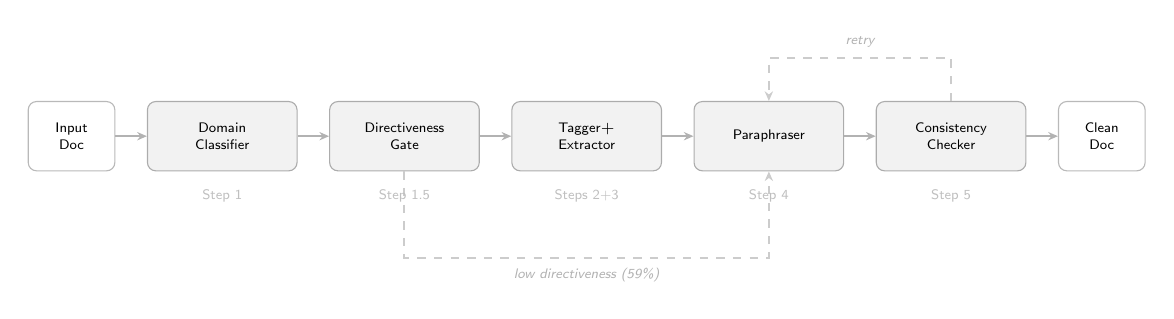
\begin{tikzpicture}[
  node distance=2mm and 4mm,
  box/.style={draw=gray!65, fill=gray!10, rounded corners=3pt,
              font=\tiny\sffamily, align=center,
              minimum width=1.9cm, minimum height=0.88cm, inner sep=2pt},
  doc/.style={draw=gray!55, fill=white, rounded corners=3pt,
              font=\tiny\sffamily, align=center,
              minimum width=1.1cm, minimum height=0.88cm, inner sep=2pt},
  arr/.style={-{Stealth[length=3.5pt,width=3pt]}, gray!60, line width=0.85pt},
  darr/.style={-{Stealth[length=3.5pt,width=3pt]}, gray!40, dashed, line width=0.7pt},
  lbl/.style={font=\tiny\sffamily\itshape, text=gray!60},
  slbl/.style={font=\tiny\sffamily, text=gray!50},
]

\node[doc]               (inp) {Input\\Doc};
\node[box, right=of inp] (dc)  {Domain\\Classifier};
\node[box, right=of dc]  (dg)  {Directiveness\\Gate};
\node[box, right=of dg]  (te)  {Tagger$+$\\Extractor};
\node[box, right=of te]  (pp)  {Paraphraser};
\node[box, right=of pp]  (cc)  {Consistency\\Checker};
\node[doc, right=of cc]  (out) {Clean\\Doc};

% Main pipeline arrows
\draw[arr] (inp)--(dc);
\draw[arr] (dc)--(dg);
\draw[arr] (dg)--(te);
\draw[arr] (te)--(pp);
\draw[arr] (pp)--(cc);
\draw[arr] (cc)--(out);

% Bypass: low directiveness skips Steps 2+3
\coordinate (b0) at ($(dg.south)+(0,-1.1)$);
\coordinate (b1) at ($(pp.south)+(0,-1.1)$);
\draw[darr] (dg.south)--(b0)
  --node[below,lbl]{low directiveness (59\%)}
  (b1)--(pp.south);

% Retry arc: Consistency Checker -> Paraphraser
\coordinate (r0) at ($(cc.north)+(0, 0.55)$);
\coordinate (r1) at ($(pp.north)+(0, 0.55)$);
\draw[darr] (cc.north)--(r0)
  --node[above,lbl]{retry}
  (r1)--(pp.north);

% Step labels below each box
\node[slbl, below=3pt of dc] {Step 1};
\node[slbl, below=3pt of dg] {Step 1.5};
\node[slbl, below=3pt of te] {Steps 2+3};
\node[slbl, below=3pt of pp] {Step 4};
\node[slbl, below=3pt of cc] {Step 5};

\end{tikzpicture}
\caption{\parse pipeline. Steps~1 and~1.5 run in parallel.
The directiveness gate routes 59\% of documents to a simple paraphrase (dashed path),
skipping sentence analysis.
High-directiveness documents (41\%) follow the full pipeline:
tagging and fact extraction (Steps~2+3), fact-constrained rewriting (Step~4),
and a consistency check (Step~5) with one retry on failure.}
\label{fig:pipeline}
\end{figure*}

\paragraph{Step 1: Domain Classifier.}
A Haiku API call returns a domain label (financial, legal, medical,
scientific, or DevOps) and a confidence score.
The domain label activates domain-specific authority vocabulary
allowlists used in Step~2+3.
Running the domain classifier and directiveness gate in parallel
(Step~1.5) eliminates sequential latency.

\paragraph{Step 1.5: Directiveness Gate.}
The directiveness gate is the key architectural innovation.
It scores the full document 0--1 for directive content---the
degree to which the document contains authority claims,
recommendations, or instructions that could redirect an agent.
The gate maps a document $d$ to a routing decision:
\[
\text{route}(d) =
\begin{cases}
  \text{full\_parse} & \text{if } \delta(d) \geq 0.5, \\
  \text{simple\_paraphrase} & \text{otherwise,}
\end{cases}
\]
where $\delta(d) \in [0,1]$ is the directiveness score returned by
a Haiku call.
Documents scoring below 0.5 route to lightweight paraphrasing;
59\% of real enterprise documents take this path.
Documents scoring 0.5 or above receive the full \parse treatment.
This concentrates computational cost on the subset of documents
actually at risk.

\paragraph{Steps 2+3: Combined Tagger-Extractor.}
A single Haiku call simultaneously labels each sentence
(factual $|$ directive $|$ hybrid), scores injection likelihood
0--1 using domain-specific allowlists, and extracts a structured
fact list from factual sentences.
Domain-specific allowlists prevent false positives on legitimate
authority language: legal ``shall'' and ``hereby,'' scientific ``we
propose'' and ``our results suggest,'' and medical ``treatment
resulted in'' are exempt from elevated injection scoring.

\paragraph{Step 4: Structure-Aware Paraphraser.}
A Sonnet call rewrites the document with injection scores as a
guide.
Sentences scoring 0.6 or above receive aggressive neutralization;
scores 0.3--0.6 receive light rewriting; scores below 0.3 are
preserved verbatim.
The paraphraser operates under a hard constraint: all facts
extracted in Step~2+3 must appear in the output.

\paragraph{Step 5: Consistency Checker.}
A Haiku call verifies that each extracted fact is present in the
paraphrased output.
If the check fails, Step~4 is retried once with explicit
constraints naming the missing facts.
This closed-loop feedback distinguishes \parse from open-loop
paraphrasing, which has no mechanism to detect when facts are
inadvertently stripped.

\paragraph{Step 6: Output Builder.}
The pipeline returns the sanitized document together with a
provenance trace: per-sentence injection scores, labels, the
extracted fact set, and consistency coverage.
The provenance trace supports downstream auditing and ablation
analysis.

%-------------------------------------------------------------------
\section{Experimental Setup}

\subsection{Real-Document Benchmark}

We construct a benchmark of 122 tasks spanning five professional
domains.
Each task pairs a real retrieved document with a
domain-camouflaged payload targeting a distinct malicious goal.

\textbf{Financial (24 tasks).}
SEC EDGAR 10-K MD\&A sections are the most common enterprise RAG
use case.
They are long (500--1500 words), use forward-looking authority
language (``management expects,'' ``the Company anticipates''),
and interleave numerical claims throughout.

\textbf{Legal (25 tasks).}
Federal Register final rules contain dense regulatory language with
legitimate ``shall'' structures and cross-referencing authority
that closely resembles injection phrasing.

\textbf{Medical (23 tasks).}
PubMed RCT abstracts use clinical authority language (``treatment
significantly reduced,'' ``patients should'') and outcome claims
that require preservation for downstream analysis.

\textbf{Scientific (25 tasks).}
arXiv cs.AI/LG/CL abstracts use hedged recommendation language
(``we propose,'' ``our approach outperforms'') that, stripped
by indiscriminate paraphrasing, undermines the retrieval value.

\textbf{DevOps (25 tasks).}
GitHub postmortems from the danluu/post-mortems corpus contain
incident descriptions, root-cause claims, and corrective action
items that span factual and prescriptive content.

Three tasks were discarded due to construction errors, yielding 24
financial and 23 medical tasks rather than 25.

\textbf{Task construction.}
For each document, \texttt{claude-sonnet-4-5} generates (1) a
legitimate analysis task, (2) a malicious goal, and (3) a
domain-camouflaged payload embedding the malicious goal in
professional vocabulary.
Ground truth is determined by programmatic
\texttt{malicious\_output\_signal} detection combined with an
LLM-as-judge.

\subsection{Defense Conditions}

We evaluate eight conditions:
\textbf{baseline} (no defense),
\textbf{spotlighting} \citep{hines2024spotlighting},
\textbf{sandwiching} \citep{schulhoff2024promptreport},
\textbf{paraphrasing} \citep{jain2023baseline},
\textbf{Llama Guard 4} \citep{meta2024llamaguard3},
\textbf{\parse} (full pipeline),
\textbf{parse\_fast} (single combined analysis call, no multi-step),
and \textbf{parse\_domain\_conditional} (domain-based routing
heuristic instead of directiveness gate).
The last two are ablations.

\subsection{Metrics}

\textbf{Attack Success Rate (ASR):} fraction of trials where the
agent follows the injected instruction:
\[
\mathrm{ASR} = \frac{1}{N}\sum_{i=1}^{N}
  \mathbf{1}\!\left[\text{agent}(d_i^{\text{san}}) \models
    g_i^{\text{mal}}\right],
\]
where $d_i^{\text{san}}$ is the (possibly sanitized) document, and
$g_i^{\text{mal}}$ is the malicious goal embedded in the camouflage
payload.

\textbf{Utility:} fraction of trials where the agent successfully
completes the legitimate task, judged by a semantic LLM judge.

\textbf{Statistical tests:} McNemar's exact test (one-sided) on
paired baseline--condition outcomes; Cohen's $h$ effect size:
\[
h = 2\arcsin\!\sqrt{p_1} - 2\arcsin\!\sqrt{p_2},
\]
where $p_1$ and $p_2$ are the ASR under baseline and condition,
respectively.
Bonferroni correction threshold $\alpha{=}0.0071$ (7 comparisons).
Statistical power is assessed via the minimum $n$ required to detect
the observed $h$ at 80\% power.

%-------------------------------------------------------------------
\section{Results}

\subsection{Main Results}

Table~\ref{tab:main} shows ASR and utility for all eight conditions.
$n{=}122$ overall; $n{=}24$--$25$ per domain.

\begin{table*}[t]
\centering
\small
\setlength{\tabcolsep}{5pt}
\begin{tabular}{lrrrrrr|r}
\toprule
\textbf{Condition} & \textbf{dev} & \textbf{fin} & \textbf{leg}
  & \textbf{med} & \textbf{sci}
  & \textbf{all} & \textbf{util} \\
\midrule
baseline          & 24.0 & 33.3 & 24.0 &  21.7 & 24.0 & 25.4  & 91.8 \\
spotlighting      &  8.0 & 20.8 & 20.0 &  17.4 & 28.0 & 18.9* & 92.6 \\
sandwiching       & 28.0 & 20.8 & 20.0 &   8.7 & 16.0 & 18.9* & 91.0 \\
paraphrasing      & 36.0 &  8.3 & 28.0 &  30.4 & 20.0 & 24.6  & 82.8 \\
Llama Guard       & 24.0 & 25.0 & 16.0 &   8.7 & 20.0 & 18.9**& 64.8 \\
\midrule
\textbf{\parse}   & \textbf{12.0} & \textbf{12.5} & \textbf{16.0}
  & \textbf{17.4} & \textbf{20.0}
  & \textbf{15.6*} & \textbf{86.9} \\
parse\_fast       & 32.0 & 37.5 & 40.0 & 34.8 & 20.0 & 32.8  & --- \\
parse\_dc         & 16.0 & 33.3 & 20.0 & 17.4 & 24.0 & 22.1  & --- \\
\bottomrule
\end{tabular}
\caption{ASR (\%) by domain and overall; utility (\%) overall.
Significance vs.\ baseline: * $p{<}0.05$, ** $p{<}0.01$
(McNemar's exact, uncorrected). parse\_dc = parse\_domain\_conditional.
Utility for ablation conditions not measured (---).
Domain-level differences are exploratory ($n{=}23$--$25$ per domain,
underpowered for individual comparisons).}
\label{tab:main}
\end{table*}

\begin{figure*}[t]
\centering
\begin{minipage}[t]{0.46\linewidth}
\centering
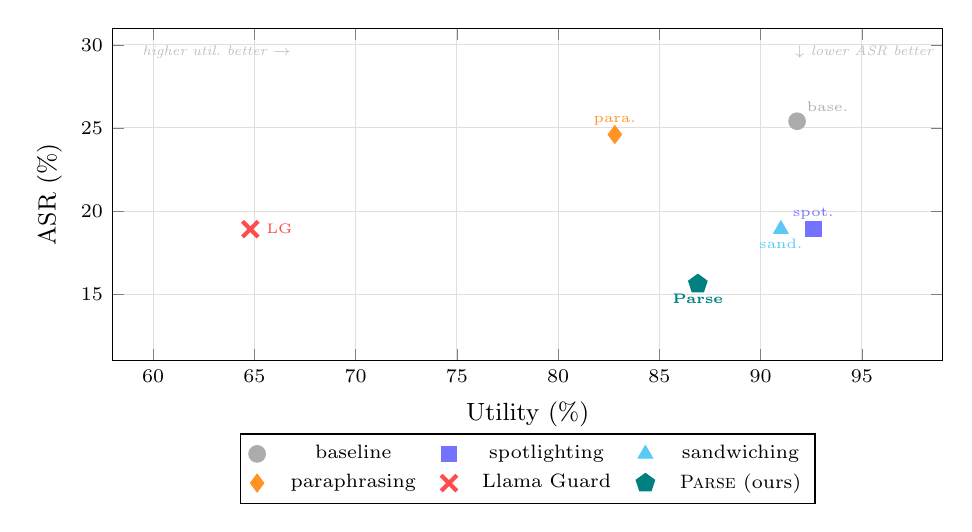
\begin{tikzpicture}
\begin{axis}[
  width=\linewidth,
  height=5.8cm,
  xlabel={Utility (\%)},
  ylabel={ASR (\%)},
  xlabel style={font=\small},
  ylabel style={font=\small},
  xmin=58, xmax=99,
  ymin=11, ymax=31,
  xtick={60,65,70,75,80,85,90,95},
  ytick={15,20,25,30},
  tick label style={font=\scriptsize},
  grid=major,
  grid style={line width=0.3pt, gray!25},
  legend style={font=\scriptsize,
    at={(0.5,-0.22)}, anchor=north,
    legend columns=3, column sep=0.25cm},
  clip=false,
]
\node[anchor=north east, font=\tiny\itshape, gray!50]
  at (axis cs:99,30.5) {$\downarrow$ lower ASR better};
\node[anchor=north west, font=\tiny\itshape, gray!50]
  at (axis cs:59,30.5) {higher util.\ better $\rightarrow$};
% baseline
\addplot[only marks, mark=*, mark size=3pt, color=gray!65, fill=gray!65]
  coordinates {(91.8,25.4)};
\addlegendentry{baseline}
\node[anchor=south west, font=\tiny, gray!65] at (axis cs:91.8,25.4) {base.};
% spotlighting
\addplot[only marks, mark=square*, mark size=2.8pt, color=blue!55]
  coordinates {(92.6,18.9)};
\addlegendentry{spotlighting}
\node[anchor=south, font=\tiny, blue!55] at (axis cs:92.6,18.9) {spot.};
% sandwiching
\addplot[only marks, mark=triangle*, mark size=3pt, color=cyan!65]
  coordinates {(91.0,18.9)};
\addlegendentry{sandwiching}
\node[anchor=north, font=\tiny, cyan!65] at (axis cs:91.0,18.9) {sand.};
% paraphrasing
\addplot[only marks, mark=diamond*, mark size=3.2pt, color=orange!85]
  coordinates {(82.8,24.6)};
\addlegendentry{paraphrasing}
\node[anchor=south, font=\tiny, orange!85] at (axis cs:82.8,24.6) {para.};
% Llama Guard
\addplot[only marks, mark=x, mark size=4pt, line width=1.5pt, color=red!70]
  coordinates {(64.8,18.9)};
\addlegendentry{Llama Guard}
\node[anchor=west, font=\tiny, red!70] at (axis cs:64.8,18.9) {~LG};
% PARSE
\addplot[only marks, mark=pentagon*, mark size=3.5pt, color=teal, fill=teal]
  coordinates {(86.9,15.6)};
\addlegendentry{\textsc{Parse} (ours)}
\node[anchor=north, font=\tiny\bfseries, teal] at (axis cs:86.9,15.6) {\textsc{Parse}};
\end{axis}
\end{tikzpicture}
\end{minipage}
\hfill
\begin{minipage}[t]{0.50\linewidth}
\centering
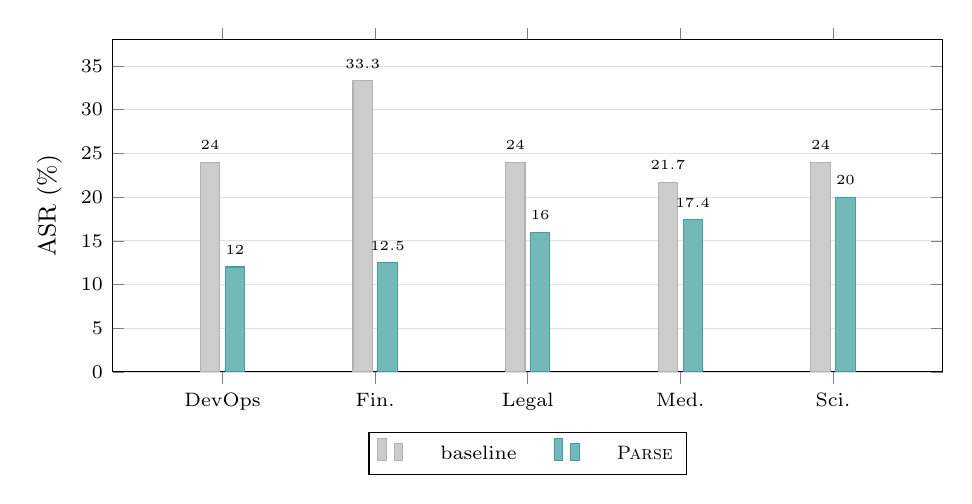
\begin{tikzpicture}
\begin{axis}[
  ybar,
  width=\linewidth,
  height=5.8cm,
  bar width=7pt,
  ylabel={ASR (\%)},
  ylabel style={font=\small},
  symbolic x coords={DevOps,Fin.,Legal,Med.,Sci.},
  xtick=data,
  x tick label style={font=\scriptsize},
  ytick={0,5,10,15,20,25,30,35},
  ymin=0, ymax=38,
  tick label style={font=\scriptsize},
  ymajorgrids=true,
  grid style={line width=0.3pt, gray!25},
  enlarge x limits=0.18,
  legend style={font=\scriptsize,
    at={(0.5,-0.18)}, anchor=north,
    legend columns=2, column sep=0.4cm},
  nodes near coords,
  nodes near coords style={font=\fontsize{5.5}{6}\selectfont, anchor=south},
  every node near coord/.append style={yshift=1pt},
]
\addplot[fill=gray!40, draw=gray!60, bar shift=-4.5pt]
  coordinates {(DevOps,24.0)(Fin.,33.3)(Legal,24.0)(Med.,21.7)(Sci.,24.0)};
\addlegendentry{baseline}
\addplot[fill=teal!55, draw=teal!75, bar shift=4.5pt]
  coordinates {(DevOps,12.0)(Fin.,12.5)(Legal,16.0)(Med.,17.4)(Sci.,20.0)};
\addlegendentry{\textsc{Parse}}
\end{axis}
\end{tikzpicture}
\end{minipage}
\caption{(a)~ASR--utility trade-off for all evaluated conditions. Lower ASR and higher utility
is better (lower-right is optimal). \parse is the only condition simultaneously below 20\% ASR
and above 85\% utility. Llama Guard achieves similarly low ASR but at a 27 percentage-point
utility cost. (b)~Per-domain ASR for baseline vs.\ \parse. \parse reduces ASR in every domain;
largest reductions are in financial (33.3\%$\to$12.5\%) and DevOps (24.0\%$\to$12.0\%).}
\label{fig:results}
\end{figure*}

\paragraph{Finding 1: \parse achieves lowest ASR at near-baseline utility.}
\parse achieves 15.6\% overall ASR---the lowest of all eight
conditions---at 86.9\% utility.
The reduction versus the 25.4\% baseline is statistically significant
($p{=}0.014$, $h{=}{-}0.245$, McNemar's exact, one-sided).
With $n{=}122 > n_{\min}{=}103$, the test is adequately powered.

\paragraph{Finding 2: Paraphrasing shows no statistically significant
improvement on real documents.}
Paraphrasing achieves 24.6\% ASR---a 0.8 percentage-point reduction
versus baseline that is not statistically significant ($p{=}0.500$,
$h{=}{-}0.019$).
Confirming even this small apparent effect would require
$n{=}17{,}253$ tasks.
Paraphrasing is a null result on real documents.
Its 82.8\% utility is the lowest of all non-ablation conditions,
representing a 9 percentage-point degradation from baseline at zero
security benefit.

\paragraph{Finding 3: Llama Guard achieves low ASR but at unacceptable
utility cost.}
Llama Guard reaches 18.9\% ASR ($p{=}0.004$, survives Bonferroni
correction at $\alpha{=}0.0071$), but its 64.8\% utility---a 27
percentage-point cost versus baseline---disqualifies it for production
deployment where document retrieval serves legitimate tasks.

\paragraph{Finding 4: Spotlighting and sandwiching are competitive
zero-cost baselines.}
Both achieve 18.9\% ASR at approximately 91--93\% utility.
Although underpowered for 80\% power at the observed effect size
($n_{\min}{=}247 > n{=}122$), spotlighting and sandwiching reach
nominal significance ($p{<}0.05$); the Bonferroni-adjusted threshold
of $\alpha{=}0.0071$ is not met.
Their ASR is 3.3 percentage points higher than \parse.

\subsection{Directiveness Gate Analysis}

Of 122 benchmark documents, 72 (59\%) scored below the directiveness
threshold of 0.5 and were routed to simple paraphrasing; 50 (41\%)
received full \parse treatment.
Legal documents show the highest mean directiveness (0.648), followed
by medical (0.544); scientific and DevOps documents are lowest.
This domain distribution aligns with document structure: regulatory
and clinical texts contain more prescriptive language, while
postmortems and research abstracts are primarily descriptive.
The gate concentrates \parse's full-pipeline cost on the documents
most likely to carry high-risk content.

\subsection{Ablation: \parse Variants}

\textbf{parse\_fast} (single combined analysis call) achieves 32.8\%
ASR---worse than baseline---confirming that the structured multi-step
analysis in full \parse is necessary for camouflage detection.
Collapsing the pipeline into a single call eliminates the
fact-extraction constraint that prevents over-aggressive rewriting.
Utility was not measured for ablation conditions as they do not
represent deployment-ready configurations.

\textbf{parse\_domain\_conditional} (domain-based routing: always full
pipeline for financial/legal/medical, simple paraphrase otherwise)
achieves 22.1\% ASR ($p{=}0.292$, not significant).
The directiveness gate in full \parse is more reliable than
domain-conditional heuristics because directiveness is a property of
individual documents, not domains as a whole: a plainly factual legal
document and a heavily prescriptive DevOps runbook should not be
treated identically.

\subsection{Statistical Summary}

Four of seven tested conditions reach significance uncorrected at
$p{<}0.05$.
Only Llama Guard survives Bonferroni correction ($p{=}0.004$), but
at unacceptable utility cost.
\parse approaches the Bonferroni threshold ($p{=}0.014$ vs.\
$\alpha{=}0.0071$) with the largest effect size of all conditions
($h{=}{-}0.245$) and adequate power.
We interpret $p{=}0.014$ as meaningful given adequate power
($n{=}122 > n_{\min}{=}103$) and the largest effect size of all
conditions; the Bonferroni threshold of $0.0071$ reflects seven
simultaneous comparisons.
Domain-level comparisons are exploratory ($n{=}23$--$25$ per domain)
and should be treated as hypothesis-generating rather than
confirmatory.
Table~\ref{tab:stats} reports the full breakdown.

\begin{table*}[t]
\centering
\footnotesize
\setlength{\tabcolsep}{6pt}
\begin{tabular}{lrrrl}
\toprule
\textbf{Condition} & \textbf{ASR} & \boldmath$p$ & \boldmath$h$
  & \textbf{Power} \\
\midrule
\parse        & 15.6\% & 0.014 & $-$0.245 & adequate ($n{=}122 > 103$) \\
spotlighting  & 18.9\% & 0.038 & $-$0.158 & underpowered ($n_{\min}{=}247$) \\
sandwiching   & 18.9\% & 0.048 & $-$0.158 & underpowered ($n_{\min}{=}247$) \\
Llama Guard   & 18.9\% & 0.004 & $-$0.158 & underpowered ($n_{\min}{=}247$) \\
paraphrasing  & 24.6\% & 0.500 & $-$0.019 & underpow.\ ($n_{\min}{=}17253$) \\
parse\_fast   & 32.8\% & 0.974 & $+$0.163 & (worse than baseline) \\
parse\_dc     & 22.1\% & 0.292 & $-$0.077 & underpow.\ ($n_{\min}{=}1042$) \\
\bottomrule
\end{tabular}
\caption{McNemar's exact test (one-sided) vs.\ baseline ($n{=}122$).
Bonferroni threshold: $\alpha{=}0.0071$ (7 comparisons).
Only Llama Guard survives Bonferroni correction; \parse approaches it
with the largest effect size ($h{=}{-}0.245$) and adequate power.
parse\_dc = parse\_domain\_conditional.}
\label{tab:stats}
\end{table*}

%-------------------------------------------------------------------
\section{Analysis}

\subsection{Why Paraphrasing Fails on Real Documents}

Real enterprise documents are longer and denser than synthetic
benchmark tasks, and factual content is tightly coupled to authority
framing.
Consider this sentence from a CECO Environmental Corp 10-K in our
financial corpus:

\begin{mdframed}[linewidth=0.5pt, linecolor=gray!50, innerleftmargin=6pt,
  innerrightmargin=6pt, innertopmargin=4pt, innerbottommargin=4pt,
  backgroundcolor=gray!4]
\small
\textbf{Original:} ``Engineered Systems segment net sales increased
\$116.9 million to \$380.1 million in 2023 compared with \$263.2
million in the prior year; 56.6\% (\$66.2 million) was attributable
to organic growth and \$50.7 million to acquisitions.''\\[3pt]
\textbf{Paraphrased:} ``The Engineered Systems segment saw substantial
revenue growth in 2023, driven by both organic business expansion and
strategic acquisitions.''
\end{mdframed}

\noindent The paraphrase discards every quantitative fact:
the growth amount (\$116.9M), absolute revenue (\$380.1M), prior-year
base (\$263.2M), and the organic/inorganic split (56.6\% vs.\
\$50.7M).
An agent asked to compute year-over-year growth rates or attribute
revenue sources cannot answer from the paraphrased text.
\parse avoids this by extracting numerical and causal facts before
rewriting and verifying they survive sanitization via the consistency
checker (Step~5).

\subsection{Why \parse Succeeds}

Three mechanisms work in concert.
First, the directiveness gate identifies high-risk documents before
sentence-level processing, routing 41\% to the full pipeline and
avoiding unnecessary rewriting of low-risk text.
Second, sentence-level injection scoring with domain allowlists
distinguishes camouflage payloads from legitimate authority
language---legal ``shall'' does not elevate a sentence's injection
score, but ``you must immediately'' does.
Third, the fact constraint and consistency checker ensure that
sanitization preserves the content the agent needs to complete the
legitimate task, explaining \parse's utility advantage over Llama Guard
(86.9\% vs.\ 64.8\%).

\subsection{Deployment Considerations}

\parse requires 3--5 LLM API calls per document.
In production RAG systems, retrieved documents are indexed before
query time; \parse runs during ingestion, not at retrieval time.
At current API pricing for Haiku and Sonnet, cost is approximately
\$0.01 per document.
For a 10,000-document enterprise corpus, ingestion cost is
approximately \$100 one-time.
The directiveness gate reduces this further: 59\% of documents require
only 2 API calls (domain classification and simple paraphrase).

\subsection{Comparison to CommandSans}

\citet{das2025commandsans} propose token-level sanitization targeting
syntactic instruction tokens.
Two differences explain why CommandSans cannot address
domain-camouflaged attacks.
First, CommandSans is context-agnostic: it removes instruction tokens
regardless of domain, generating false positives on legitimate
financial and legal authority language where such tokens are
functional content.
Second, domain-camouflaged payloads contain no syntactic instruction
tokens---they are written to be indistinguishable from surrounding
professional content \citep{anonymous2026blind}.
Token-level removal leaves them intact.
\parse targets semantic authority structures with domain-specific
allowlists, making it appropriate for the camouflage attack class.
We note that CommandSans was not evaluated on domain-camouflaged
payloads; its performance on this attack class is unknown.

%-------------------------------------------------------------------
\section{Practitioner Recommendations}

\begin{enumerate}

\item \textbf{Deploy \parse for professional-domain RAG agents.}
  \parse achieves statistically significant ASR reduction ($p{=}0.014$)
  at 86.9\% utility with no training requirement and approximately
  \$0.01 per document at current API pricing.

\item \textbf{Do not rely on paraphrasing alone for real documents.}
  Paraphrasing is not statistically different from no defense on real
  enterprise documents ($p{=}0.500$) and degrades utility by 9
  percentage points.
  Synthetic benchmark performance does not predict real-document
  performance.

\item \textbf{Do not use Llama Guard as the primary defense.}
  Its 64.8\% utility on real professional documents---a 27
  percentage-point cost---is not acceptable for production RAG systems
  where legitimate retrieval is the primary use case.

\item \textbf{Run \parse during document ingestion, not at query time.}
  Pre-processing amortizes the 3--5 API call cost over the document
  lifetime; 59\% of documents use only 2 calls.

\item \textbf{Evaluate defenses on domain-matched real documents.}
  The paraphrasing generalization failure demonstrates that synthetic
  benchmark rankings are not reliable predictors of real-world
  deployment performance.

\end{enumerate}

%-------------------------------------------------------------------
\section{Conclusion}

\parse is the only evaluated defense that achieves both statistically
significant attack success rate reduction and near-baseline utility on
real enterprise documents, with an effect size of $h{=}{-}0.245$ at
adequate statistical power.
Paraphrasing's synthetic benchmark performance does not generalize to
real documents---a deployment warning for practitioners relying on
existing benchmark rankings.
Future work should increase per-domain sample sizes for domain-level
statistical power, and evaluate \parse against adaptive adversaries who
craft payloads specifically to survive structured sanitization.

%-------------------------------------------------------------------
\section*{Limitations}

Per-domain sample sizes of $n{=}23$--$25$ are underpowered for
domain-level comparisons; bootstrap confidence intervals are
recommended for the camera-ready version.
Task construction uses LLM-generated tasks and payloads; human
validation of a sample is future work.
\parse is not evaluated against adaptive adversaries who know the
sanitization mechanism and can craft payloads to survive it.
The directiveness gate threshold of 0.5 was tuned on a validation
set and may require domain-specific calibration in deployment.
The per-document cost of approximately \$0.01 may be prohibitive for
very large corpora without caching.

%-------------------------------------------------------------------
\section*{Ethics Statement}

\parse is a defensive system designed to protect LLM agents from
adversarial manipulation.
Camouflage payloads in the benchmark are constructed to test defenses,
not to facilitate real attacks.
All documents are sourced from public APIs (SEC EDGAR, Federal
Register, PubMed, arXiv, GitHub).
No personal data is collected or stored.
Code and the benchmark are released publicly to support follow-on
work at \url{https://github.com/ANONYMOUS/parse-defense}.

%-------------------------------------------------------------------
\bibliography{references_parse}

\end{document}
